\section{Experiment}

\subsection*{Data}
\begin{figure}[H]
	\centering
	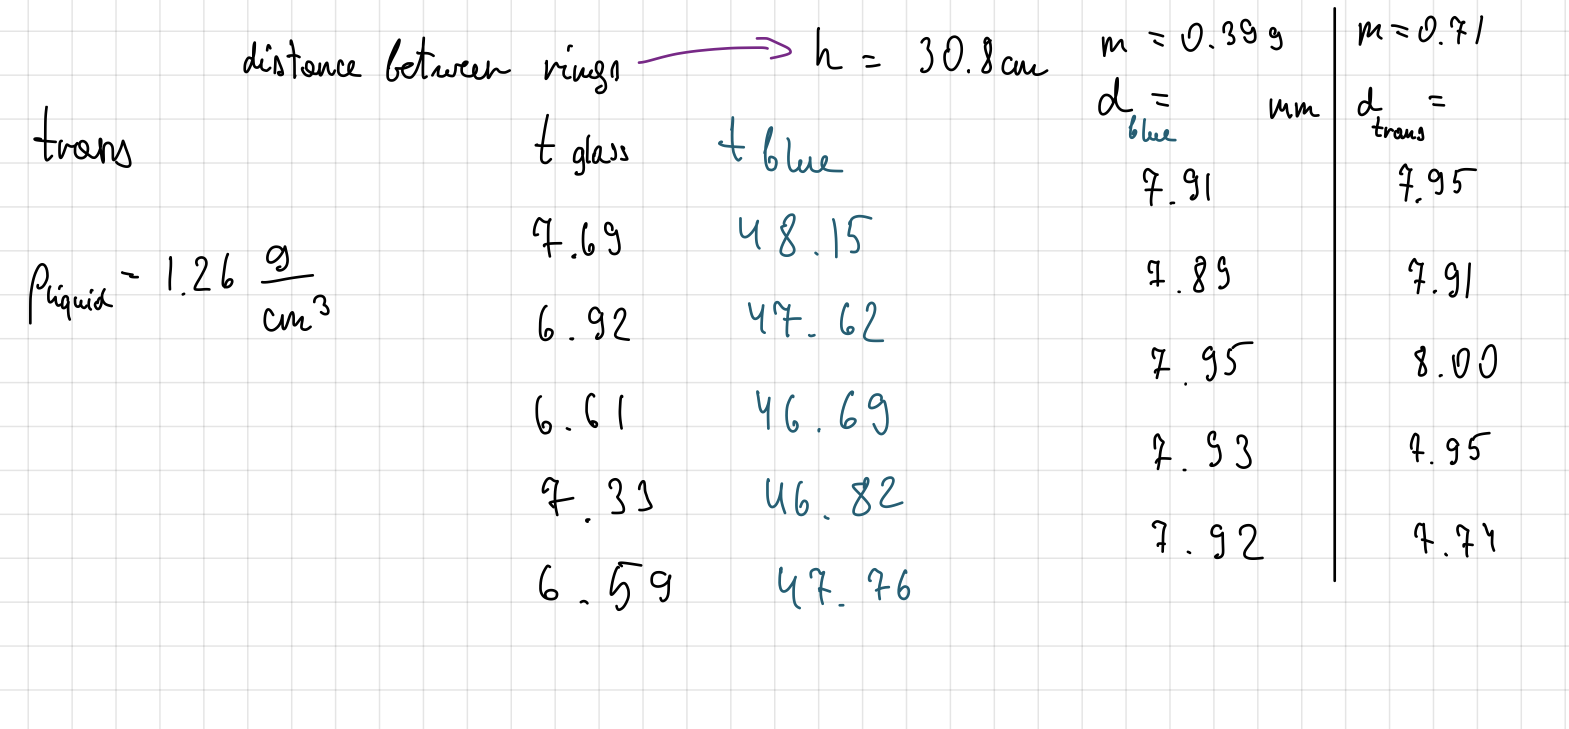
\includegraphics[width=12cm]{schematics/data.png}
	\caption{Experiment data}
\end{figure}

\begin{table}[H]
    \centering
    \begin{tabular}{|l|l|l|l|l|}
    \hline
    lp. & m [kg] & d [m] & h [m] & t [s]\\ \hline
    1 & 0.000399 & 0.00791 & 0.308 & 48.15 \\ \hline
        2 & ~ & 0.00789 & ~ & 47.62 \\ \hline
        3 & ~ & 0.00795 & ~ & 46.69 \\ \hline
        4 & ~ & 0.00793 & ~ & 46.82 \\ \hline
        5 & ~ & 0.00792 & ~ & 47.76 \\ \hline
        X & ~ & 0.00792 & ~ & 47.408 \\ \hline
        $\Delta_p$ & 0.0000001 & 0.00001 & 0.001 & 0.01 \\ \hline
        ua(X) & ~ & 0.00001 & ~ & 0.2812 \\ \hline
        ub(X) & 0.000000058 & 0.0000058 & 0.00058 & 0.0058 \\ \hline
        u(X) & 0.000000058 & 0.0000116 & 0.00058 & 0.2813 \\ \hline
        uc(X) & ~ & ~ & ~ & ~ \\ \hline
        n & 0.1367207265 & ~ & ~ & ~ \\ \hline
        u(n) & 0.0012 & & & \\ \hline
        uc(X) & ~ & ~ & ~ & ~ \\ \hline
        $\eta$ & 0.1367207265 & ~ & ~ & ~ \\ \hline
        u($\eta$) & 0.0012 & & & \\ \hline
        ~ & ~ & ~ & ~ & ~ \\ \hline
        ~ & $\rho$k[kg/m\^2] & $\rho$c[kg/m\^3] & $\eta$[Ns/m\^2] & ~ \\ \hline
        ~ & 1533.905938 & 1260 & 0.1385153566 & ~ \\ \hline
        ~ & ~ & ~ & 0.1362988097 & ~ \\ \hline
        ~ & ~ & ~ & 0.1356771765 & ~ \\ \hline
        ~ & ~ & ~ & 0.1353712533 & ~ \\ \hline
        ~ & ~ & ~ & 0.1377410366 & ~ \\ \hline
        ~ & ~ & ~ & ~ & ~ \\ \hline
        uc(X) & 6.8 & ~ & 0.0096 \\ \hline
    \end{tabular}
    \caption{Blue ball}
\end{table}

\begin{table}[H]
    \centering
    \begin{tabular}{|l|l|l|l|l|}
    \hline
    lp. & m [kg] & d [m] & h [m] & t [s]\\ \hline
        1 & 0.00071 & 0.00795 & 0.308 & 7.69 \\ \hline
        2 & ~ & 0.00791 & ~ & 6.92 \\ \hline
        3 & ~ & 0.008 & ~ & 6.61 \\ \hline
        4 & ~ & 0.00795 & ~ & 7.33 \\ \hline
        5 & ~ & 0.00774 & ~ & 6.59 \\ \hline
        X & ~ & 0.00791 & ~ & 7.028 \\ \hline
        $\Delta_p$ & 0.0000001 & 0.00001 & 0.001 & 0.01 \\ \hline
        ua(X) & ~ & 0.00005 & ~ & 0.2131 \\ \hline
        ub(X) & 0.000000058 & 0.0000058 & 0.00058 & 0.0058 \\ \hline
        u(X) & 0.000000058 & 0.0000504 & 0.00058 & 0.2132 \\ \hline
        uc(X) & ~ & ~ & ~ & ~ \\ \hline
        n & 0.0202312096 & ~ & ~ & ~ \\ \hline
        u(n) & 0.0013  & ~ & ~ & ~ \\ \hline
        u($\eta$) & 0.0013 & & & \\ \hline
        ~ & $\rho$k[kg/m\^2] & $\rho$c[kg/m\^3] & n[Ns/m\^2] & ~ \\ \hline
        ~ & ~ & ~ & ~ & ~ \\ \hline
        ~ & 2739.872011 & 1260 & 0.02234648719 & ~ \\ \hline
        ~ & ~ & ~ & 0.01990708759 & ~ \\ \hline
        ~ & ~ & ~ & 0.01945046997 & ~ \\ \hline
        ~ & ~ & ~ & 0.02130035775 & ~ \\ \hline
        ~ & ~ & ~ & 0.01815164552 & ~ \\ \hline
        ~ & ~ & ~ & ~ & ~ \\ \hline
        uc(X) & 12.1 & ~ & 0.0379 & \\ \hline
    \end{tabular}
    \caption{Blue ball}
\end{table}
\subsection{Formulas}

Calculating the average time of ball falling:
\begin{equation*}
	\bar{t} = \frac{t_1 + t_2 + \cdots + t_{10}}{10}
\end{equation*}

Calculating the average diameter of the ball:
\begin{equation*}
	\bar{d} = \frac{d_1 + d_2 + \cdots + d_{10}}{10}
\end{equation*}


Calculating the density of the ball:

\begin{equation*}
	\rho_k = \frac{6m}{\pi d^3}
\end{equation*}

Calculating the average coefficient of viscosity:
\begin{equation*}
	\eta = \frac{d^2 g t (\rho_k - \rho_c)}{18h}
\end{equation*}
Calculating the uncertainty of the mass measurement:

\begin{equation*}
	u(X) = \frac{\Delta_p}{\sqrt{3}}
\end{equation*}

\begin{equation*}
	u(m) = \frac{0.0000001}{\sqrt{3}} \approx 5.8 \times 10^{-8} \text{ kg}
\end{equation*}

Calculating the uncertainty of the density measurement:
\begin{equation*}
	u_c(\rho_k) = \sqrt{\left(\frac{6}{\pi d^3} u(m)\right)^2 + \left(\frac{-18m}{\pi d^4} u(d)\right)^2}
\end{equation*}

Calculating the uncertainty of the coefficient of viscosity:

\begin{equation*}
	u_c(\eta) = \sqrt{\left(\frac{2dgt(\rho_k-\rho_c)}{18h} u(d)\right)^2 + \left(\frac{d^2 g(\rho_k-\rho_c)}{18h} u(t)\right)^2}
\end{equation*}

\subsection{Calculations}
\begin{figure}[H]
	\centering
	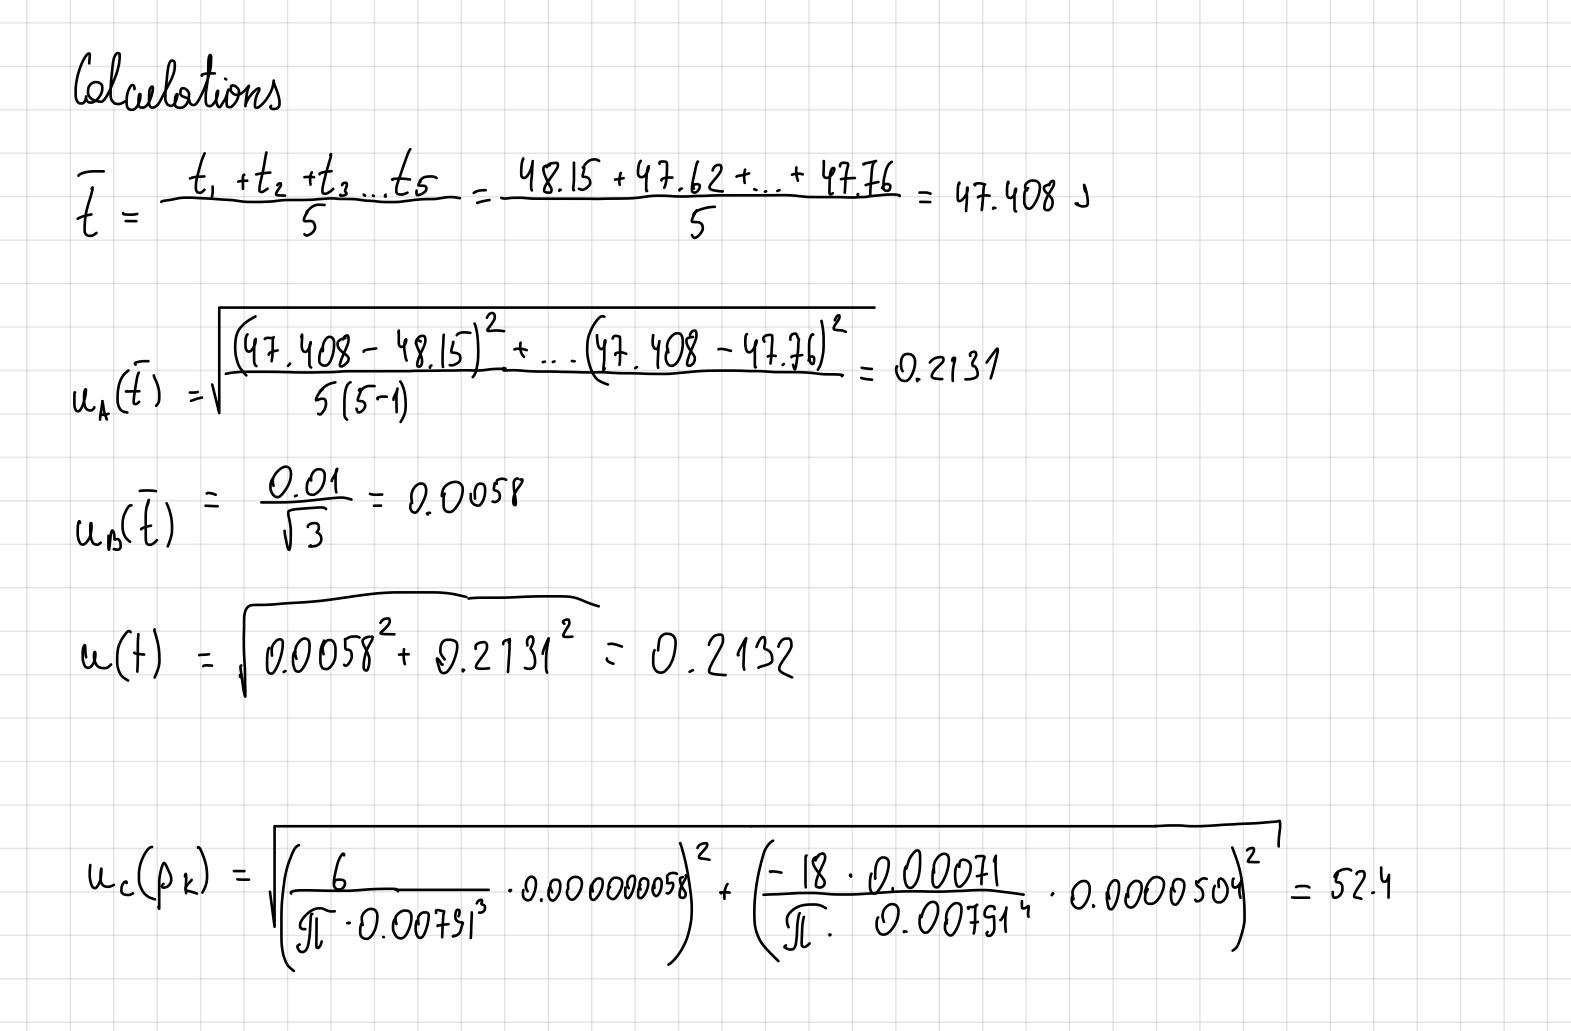
\includegraphics[width=14cm]{schematics/calculations.png}
	
\end{figure}
